\documentclass[11pt]{article}
\usepackage{fullpage}
\usepackage{amsmath}
\usepackage{amssymb}
\usepackage{graphicx}
\usepackage{color}
\usepackage{float}
\usepackage{caption}
\usepackage{cases}
\usepackage{placeins}

%\newcommand{\fb}{f_b^3}
\newcommand{\fb}[1]{f_b^{#1}}

\newcommand{\mSbFb}[1]{\mu_{s_{b} \rightarrow \fb{#1}}}
\newcommand{\mFbSb}[1]{\mu_{ \fb{#1} \rightarrow s_{b}}}

\newcommand{\mFbRb}[1]{\mu_{ \fb{#1} \rightarrow r_{b}}}
\newcommand{\mRbFb}[1]{\mu_{ r_{b} \rightarrow  \fb{#1}}}

\newcommand{\mFbGbk}[1]{\mu_{ \fb{#1} \rightarrow g_{b,k}}}
\newcommand{\mGbkFb}[1]{\mu_{  g_{b,k} \rightarrow \fb{#1}}}

\begin{document}

\title{BP}
\maketitle

\section{Model}

The atomic unit of the factor graph is shown in Figure \ref{bpModel}.

\begin{figure}[htbp]
\begin{center}
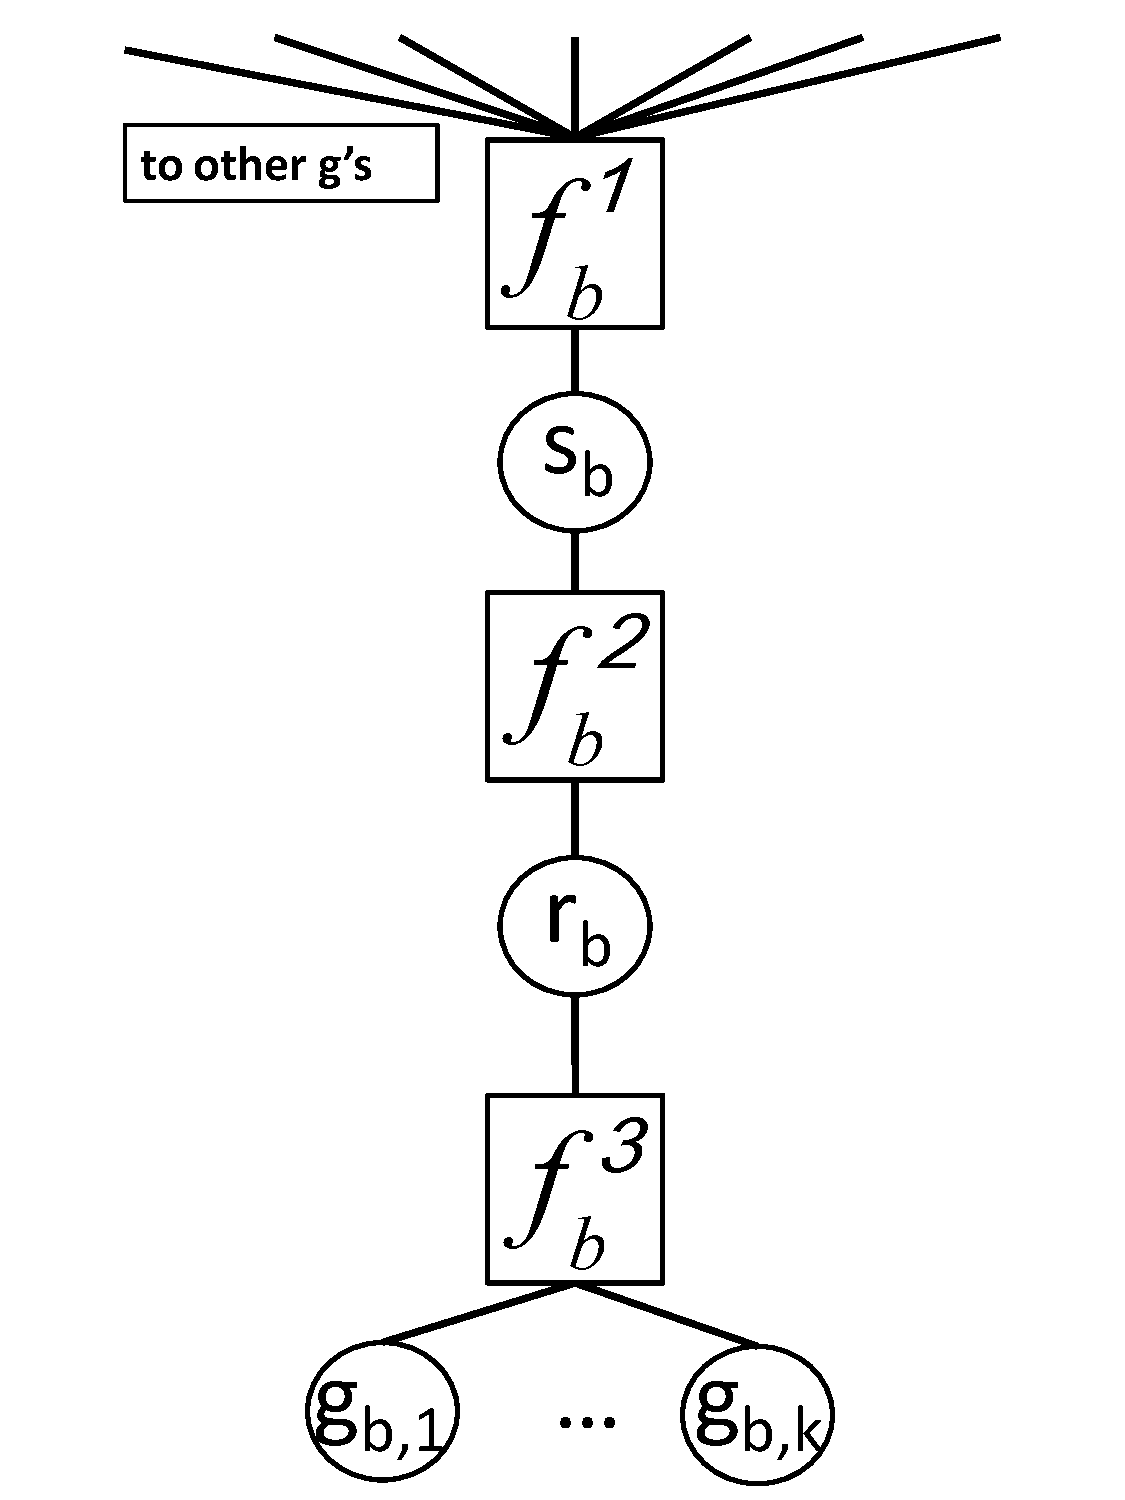
\includegraphics[width=0.5\textwidth]{bpModel.pdf}
\caption{Factor graph}
\label{bpModel}
\end{center}
\end{figure}

\FloatBarrier

We require efficient computation of the messages.

\section{Top-down messages}

\subsection{$\mFbSb1$}

The general form of the message is given by
\begin{eqnarray}
\mFbSb1(s_b) &=& \sum_{\vec{g}} \fb1(s_b, \vec{g}) \prod_{g_{b',k}} \mu_{g_{b',k} \rightarrow \fb1}(g_{b',k})
\end{eqnarray}

We divide the cases into  $s_b=0$, and  $s_b=1$.

\begin{eqnarray}
\mFbSb1(s_b=0) &=& \sum_{\vec{g}} \fb1(s_b=0, \vec{g}) \prod_{g_{b',k}} \mu_{g_{b',k} \rightarrow \fb1}(g_{b',k}) \\
&=&  (1-\epsilon) \prod_{g_{b',k}} \mu_{g_{b',k} \rightarrow \fb1}(g_{b',k}=0)
\end{eqnarray}

\begin{eqnarray}
\mFbSb1(s_b=1) &=& \sum_{\vec{g}} \fb1(s_b=1, \vec{g}) \prod_{g_{b',k}} \mu_{g_{b',k} \rightarrow \fb1}(g_{b',k}) \\
&=&  \epsilon \times \prod_{g_{b',k}} \mu_{g_{b',k} \rightarrow \fb1}(g_{b',k}=0)  \\
& & + \sum_{\vec{g}}  \prod_{g_{b',k}} \mu_{g_{b',k} \rightarrow \fb1}(g_{b',k}) - \prod_{g_{b',k}} \mu_{g_{b',k} \rightarrow \fb1}(g_{b',k}=0) \nonumber \\
&=& \epsilon \times \prod_{g_{b',k}} \mu_{g_{b',k} \rightarrow \fb1}(g_{b',k}=0)  \\
& & +1 - \prod_{g_{b',k}}  \mu_{g_{b',k} \rightarrow \fb1}(g_{b',k}=0) \nonumber \\
&=&  \prod_{g_{b',k}} \mu_{g_{b',k} \rightarrow \fb1}(g_{b',k}=0) (\epsilon -1 ) +1 \\
&=&  1- (1-\epsilon) \prod_{g_{b',k}} \mu_{g_{b',k} \rightarrow \fb1}(g_{b',k}=0) \\
&=&  1- \mFbSb1(s_b=0)
\end{eqnarray}

where we have made use of the property that messages from a node/factor sum to $1$

\subsection{$\mSbFb2$}

if $s_b$ has not been observed, this message is given by
\begin{eqnarray}
\mSbFb2(s_b) = \mFbSb1(s_b)
\end{eqnarray}
otherwise, it is a constant message that indicates its observed state.

\subsection{ $\mFbRb2$}

\begin{eqnarray}
\mFbRb2(r_b) &=& \sum_{s_b} \fb2(s_b,r_b) \mSbFb2(s_b) \\
&=& \sum_{s_b} P(r_b \mid s_b)  \mSbFb2(s_b)
\end{eqnarray}

$s_b$ only has two values, so this is easy to compute.

\subsection{$\mRbFb3$}

\begin{eqnarray}
\mRbFb3(r_b)  = \mFbRb2(r_b)
\end{eqnarray}

\subsection{$\mFbGbk3$}

\begin{eqnarray}
\mFbGbk3(g_{b,k}) &=& \sum_{r_b} \sum_{k' \neq k} \fb3(r_b,\vec{g}_b) \mRbFb3(r_b) \prod_{k' \neq k} \mGbkFb3(g_{b,k'}) \\
&=& \sum_{r_b} \mRbFb3(r_b) \sum_{k' \neq k}P(\vec{g}_b \mid r_b)  \prod_{k' \neq k}  \mGbkFb3(g_{b,k'}) \\
&=& \sum_{r_b} \mRbFb3(r_b) \sum_{k' \neq k} P(\vec{g}_{b,k} \mid r_b)  \prod_{k' \neq k} P(\vec{g}_{b,k'} \mid r_b)  \mGbkFb3(g_{b,k'}) \\
&=& \sum_{r_b} \mRbFb3(r_b)  P(\vec{g}_{b,k} \mid r_b) \prod_{k' \neq k} \sum_{g_{b,k'}}  P(\vec{g}_{b,k'} \mid r_b)  \mGbkFb3(g_{b,k'})
\end{eqnarray}

The number of values $r_b$ can take should be small (no more than, say $10$? $20$?), so this should be possible to compute.

\subsection{$\mGbkFb1$}

\begin{eqnarray}
\mGbkFb1(g_{b,k}) &=& \mFbGbk3(g_{b,k}) \prod_{b' \neq b} \mu_{f_{b'}^1 \rightarrow g_{b,k}}(g_{b,k})
\end{eqnarray}

\section{Bottom-up messages}


\subsection{$\mu_{\fb1 \rightarrow g_{b',k}}$}

Recall that $\fb1$ connects to other bricks. We denote one such brick by $b'$.

Because $\fb1$ only cares about whether $g_{b',k}$ points to $b$, we reduce the domain of $g_{b',k}$ to $0,1$ which means ``doesn't point to $b$'' and ``points to $b$'', respectively. The messages can be ``expanded'' by $g_{b',k}$ to its original domain when $g_{b',k}$ needs to send a message to $\fb3$.

The general form of this message is
\begin{eqnarray}
\mu_{\fb1 \rightarrow g_{b',k}}(g_{b,k'}) &=& \sum_{s_b} \sum_{g \neq g_{b',k}} \fb1(s_b,\mathbf{g}) \mSbFb1(s_b) \prod_{g \neq g_{b',k}} \mu_{g \rightarrow \fb1}(g).
\end{eqnarray}

We divide the cases into  $g_{b',k}=0$, and  $g_{b',k}=1$

\begin{eqnarray}
\mu_{\fb1 \rightarrow g_{b',k}}(g_{b',k}=0) &=& \mSbFb1(s_b=0) \times (1-\epsilon)  \times   \prod_{g \neq g_{b',k}}\mu_{g \rightarrow \fb1}(g=0) \\
& & +  \mSbFb1(s_b=1) \times \epsilon \times \prod_{g \neq g_{b',k}}\mu_{g \rightarrow \fb1}(g=0) \nonumber \\
& & +  \mSbFb1(s_b=1) (\prod_{g \neq g_{b',k}}\sum_{g} \mu_{g \rightarrow \fb1}(g) - \prod_{g \neq g_{b',k}} \mu_{g \rightarrow \fb1}(g=0) )  \nonumber \\
%
&=&  \mSbFb1(s_b=0) \times (1-\epsilon)  \times  \prod_{g \neq g_{b',k}}\mu_{g \rightarrow \fb1}(g=0) \\
& & + \epsilon \times \mSbFb1(s_b=1) \prod_{g \neq g_{b',k}}\mu_{g \rightarrow \fb1}(g=0) \nonumber \\
& & +  \mSbFb1(s_b=1) (1 - \prod_{g \neq g_{b',k}} \mu_{g \rightarrow \fb1}(g=0)) \nonumber \\
%
&=& \mSbFb1(s_b=0) \times (1-\epsilon)  \times  \prod_{g \neq g_{b',k}}\mu_{g \rightarrow \fb1}(g=0) \nonumber \\
& & +  \mSbFb1(s_b=1) \big(   \prod_{g \neq g_{b',k}} \mu_{g \rightarrow \fb1}(g=0)  (\epsilon -1) + 1)  \big) \\
&=&   \mSbFb1(s_b=0) \times (1-\epsilon)  \times \frac{ \prod_{g}\mu_{g \rightarrow \fb1}(g=0)}{\mu^0_{g_{b',k} \rightarrow \fb1}(g=0)}  \\
& & + \mSbFb1(s_b=1) \big( \frac{\prod_{g} \mu_{g \rightarrow \fb1}(g=0) }{\mu^0_{g_{b',k} \rightarrow \fb1}(g=0) }
 (\epsilon -1) + 1)  \big) \nonumber \\
&=&   \mSbFb1(s_b=0)  \times \frac{\mFbSb1(s_b=0)}{\mu^0_{g_{b',k} \rightarrow \fb1}(g=0)}  \\
& & + \mSbFb1(s_b=1) \times \big(1- \frac{\mFbSb1(s_b=0)}{\mu^0_{g_{b',k} \rightarrow \fb1}(g=0)}  \big) \nonumber
\end{eqnarray}

where  $\mu^0_{g_{b',k} \rightarrow \fb1}$ means the old message sent by $g_{b',k}$, and we have made use of the property that messages from a node/factor sum to $1$. Note that we can compute this message without having to explicitly examine all the other $g_{b,k}'s$; we re-used the computation from computing $\mSbFb1(s_b=0)$.

\begin{eqnarray}
\mu_{\fb1 \rightarrow g_{b',k}}(g_{b,k'}=1) &=& \mSbFb1(s_b=1) \prod_{g \neq g_{b',k}} \sum_{g}  \mu_{g \rightarrow \fb1}(g) \\
&=&  \mSbFb1(s_b=1) 
\end{eqnarray}

\subsection{$\mGbkFb3$}

\begin{eqnarray}
\mGbkFb3(g_{b,k}) = \prod_{b' \in V(b)} \mu_{f_{b'}^3 \rightarrow g_{b,k}}(g_{b,k})
\end{eqnarray}

wher $V(b)$ is the after set of brick $b$. Note that $ \mu_{f_{b'}^3 \rightarrow g_{b,k}}(g_{b,k})$ needs to be ``expanded'' to the proper domain of $g_{b,k}$

\subsection{$\mFbRb3$}

\begin{eqnarray}
\mFbRb3(r_{b}) &=& \sum_{\vec{g}} \fb3(\vec{g},r_b) \prod_{k} \mGbkFb3(g_{b,k}) \\
&=& \sum_{\vec{g}}\prod_{k} P(g_{b,k} \mid r_b) \prod_{k} \mGbkFb3(g_{b,k}) \\
&=&\prod_{k} \sum_{g_{b,k}} P(g_{b,k} \mid r_b) \mGbkFb3(g_{b,k})
\end{eqnarray}

\subsection{$\mRbFb2$}

\begin{eqnarray}
\mRbFb2(r_b) = \mFbRb3(r_b)
\end{eqnarray}

\subsection{$\mFbSb2$}

\begin{eqnarray}
\mFbSb2(s_b) &=& \sum_{r_b} \fb2(r_b,s_b) \mRbFb2(r_b) \\
&=&  \sum_{r_b} P(r_b \mid s_b) \mRbFb2(r_b)
\end{eqnarray}

These messages should be trivial to compute, since the set of values $r_b$ is small.

\subsection{$\mSbFb1$}

\begin{eqnarray}
\mSbFb(s_b) = \mFbSb2(s_b)
\end{eqnarray}

\end{document}
